% !TEX root = fa11-final.tex
\q{15}{Question Menagerie}


\begin{minipage}{0.65\linewidth}
\paragraph{Parts (a) and (b)} The hive of insects needs your help again. As before, you control an insect in a rectangular maze-like environment with dimensions $M \times N$, as shown to the right. At each time step, the insect can move into a free adjacent square or stay in its current location.  All actions have cost 1.
\\

In this particular case, the insect must pass through a series of partially flooded tunnels.  Flooded squares are lightly shaded in the example map shown.  The insect can hold its breath for $A$ time steps in a row.  Moving into a flooded square requires your insect to expend 1 unit of air, while moving into a free square refills its air supply.
\end{minipage}
\begin{minipage}{0.35\linewidth}
\begin{center}
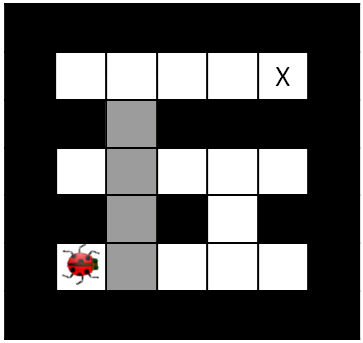
\includegraphics[width=1.8in]{figs/search}
\end{center}
\end{minipage}

\begin{enumerate}

\subq{4} Give a minimal state space for this problem (i.e. do not include extra information). You should answer for a general instance of the problem, not the specific map shown. \\

\fbox{\begin{minipage}[t][4cm][t]{13cm} \AnswerOneA \end{minipage}} \\

\subq{4} Give the size of your state space. \\

\fbox{\begin{minipage}[t][4cm][t]{13cm} \AnswerOneB \end{minipage}} \\

\suspend{enumerate}
\newpage
\textbf{Parts (c), (d), and (e)} Consider a search problem where all edges have cost 1
and the optimal solution has cost $C$.  Let $h$ be a heuristic which is $\max
\{h^* - k, 0\}$, where $h^*$ is the actual cost to the closest goal and $k$ is a
nonnegative constant.

\resume{enumerate}
\subq{3} Which of the following statements are true?\\
\begin{enumerate}[(i)]
\item $h$ is admissible. 

\item $h$ is consistent.

\item A$^*$ tree search (no closed list) with $h$ will be optimal.

\item A$^*$ graph search (with closed list) with $h$ will be optimal.

\fbox{\begin{minipage}[t][2.5cm][t]{13cm} \AnswerOneC \end{minipage}}\\

\end{enumerate}

\subq{2} Which of the following is the most reasonable description of how much
more work will be done (= how many more nodes will be expanded) with heuristic
$h$ compared to $h^*$, as a function of $k$?
\begin{enumerate}[(i)]
\item Constant in $k$\\
\item Linear in $k$\\
\item Exponential in $k$\\
\item Unbounded\\

\fbox{\begin{minipage}[t][2.5cm][t]{13cm} \AnswerOneD \end{minipage}}\\
\end{enumerate}


%\subq{1} Give an expression for the typical number of additional nodes that an A$^*$ search will expand using $h$ rather than $h^*$.  Your answer should depend on the quantities given and the branching factor $b$ of the graph.  Reminder: all edges have cost 1.
%\solution{\vspace{20mm}}{$O(b^k)$\vspace{10mm}}

%%%%%%%%%%%%%%%%%%%%%%%

\suspend{enumerate}

Now consider the same search problem, but with a heuristic $h'$ which is 0 at all states that lie along an optimal path to a goal and $h^*$ elsewhere.

\resume{enumerate}

\subq{3} Which of the following statements are true?\\
\begin{enumerate}[(i)]
\item $h'$ is admissible.\\
\item $h'$ is consistent.\\
\item A$^*$ graph search (no closed list) with $h'$ will be optimal.\\
\item A$^*$ graph search (with closed list) with $h'$ will be optimal.\\
\fbox{\begin{minipage}[t][2.5cm][t]{13cm} \AnswerOneE \end{minipage}}\\
\end{enumerate}

\end{enumerate}
